\documentclass[twocolumn, 5p, times]{elsarticle} 


\usepackage{amsmath}



\begin{document}

\title{Implementation of XIOS in the Atmospheric Component of the Unified Model}

\author[ncas,met,comp]{Bryan Lawrence}
\author[ncas,met]{Grenville Lister}
\author[ncas,met]{Jeff Cole}
\author[epcc]{Rupert Nash}
\author[epcc]{Michele Weiland}
\address[ncas]{National Centre for Atmospheric Science, UK}
\address[met]{Department of Meteorology, University of Reading, UK}
\address[comp]{Department of Computer Science, University of Reading, UK}
\address[epcc]{EPCC, The University of Edinburgh, UK}

\begin{abstract}
Weather and climate science make heavy use of ensembles of model simulations to provide an estimation of uncertainty arising from a range of causes (e.g. \cite{HawSut09}). Current practice is to write each ensemble member (simulation) out to disk as it is running and carry out an ensemble analysis at the end of the simulation. Such analysis will include simple statistics and detailed analysis of some ensemble members. However, as model resolutions increase (with more data per simulation) and ensemble sizes increase (more instances), the storage and analysis of this data are becoming prohibitively expensive -- many major weather and climate sites are looking at managing over an exabyte of data within the next few years. These costs become problematic for an environment where we anticipate running such ensembles on exascale machines, which may not include local storage of sufficient size where data can be resident for long periods of analysis.

There are only two possible strategies to cope with this data deluge -- data compression (including ``thinning'', that is, the removal of data from the output) and in-flight analysis. We discuss here some first steps with the latter approach. We exploit the XML IO server (XIOS, \cite{XIOS12}) to manage the output from simulations and to carry out some initial analysis en-route to storage.  

We have achieved three specific ambitions: (1) We have adapted a current Met Office Unified Model branch to replace much of the diagnostic system with the XIOS.
(2) We have exploited a single executable MPI environment to run multiple UM instances with output sent to XIOS, and (3) We have demonstrated that simple ensemble statistics can be calculated in-flight, including both summary statistics of individual ensemble members and cross-member statistics such as means and extremes.

With this ability, we can, in principle, avoid having all data needing to reside on a fast disk when the ensemble simulation is complete. This strategy would allow, for example, deployment on an exascale machine with burst-buffer migrating data directly to tape (or to the wide-area network). 


\end{abstract}

\begin{keyword}
ensemble
\end{keyword}

\maketitle

\section{Introduction}

As increasing computer power has become available, the weather and climate community have put effort into increasing the spatial resolution within the simulation domain, expanding the domain of simulation (spatial and temporal), expanding use of, or complexity of, data assimilation to improve initial conditions, and increasing the number of simulations within ``ensembles''. Such ensembles are collections of simulations that address the same problem, but some key aspects of each simulation differ from others. 

Ensembles typically vary along one or more of four axes: initialisation, boundary conditions, physical parameters, and modelling system (aka ``Model''). Initialisation ensembles are the mainstay of numerical weather prediction -- choosing the right set of initialisations is a science in and of itself \cite{BuiEA05}. Ensembles along the other dimensions are more typically used in climate science (e.g. the coupled model intercomparison projects such as CMIP6, \cite{MeeEA14}), but are also increasingly used at shorter timescales for weather-related problems. In all cases, the ensembles are used to sample uncertainty -- see \cite{HawSut09} for an example from climate science, and \cite{Parker10} for a more philosophical discussion of how ensembles are used to sample uncertainty.

Whatever the use, the workflows associated with ensembles are becoming problematic. When ensemble simulations run in parallel on the same platform, they can swamp the bandwidth and volume available at local storage systems. When they are run sequentially, the volume issues remain, and workflow and queuing delays become new hurdles to surmount.
 Whether simulations are run sequentially or in parallel, the current usage mode is to write out all the data from each simulation and post-process to produce ``ensemble statistics''. At many sites, this can be difficult, especially for large, long, and high-resolution ensembles.   
 Managing the workflows has become an exercise in logistics \cite{MizEA09}. These ensembles are also a significant contributor to the vast archives of data held at major weather and climate sites. Together with the cost of adequate disk, even tape archive is becoming problematic. 
 All these problems are expected to increase in the next few years, not only is there increasing scientific focus on large ensembles (e.g. \cite{YeaEA18}), problems with getting models ready for exascale \cite{LawEA18} will probably mean the first usage of exascale machines in weather and climate will be for large ensembles.

There are only two possible strategies to cope with this data deluge -- data compression (including ``thinning'', that is, the removal of data from the output) and in-flight analysis. In this paper we 
introduce some first steps with the latter approach. 
In particular, we demonstrate the use of a single executable climate ensemble system developed so that each member simulation shares access to an extra component -- an IO server -- which carries out data reductions before writing data to disk. 

Section \ref{context} discusses the climate model environment and introduces the particular IO server that is being used. Section \ref{software} introduces the software that was developed to support the ensemble system, and section \ref{results} reports on our experiences with the system. Section \ref{related} discusses related work, and in section \ref{summary} we summarise our achievements and signpost some of our plans for further work.


\section{Context}
\label{context}

Climate modelling in the UK is predominantly done using variants of the Unified Model, running standalone in ``atmosphere-only mode'' \citep{REFNEEDED}, or in coupled mode \citep{REFNEEDED}. The coupled variant is depicted in Figure \ref{coupled}: the UM atmosphere is coupled via the OASIS coupler \cite{Oasis} to a NEMO \cite{Nemo} ocean. NEMO uses the XIOS \cite{XIOS12} to write to disk, and the UM atmosphere either writes directly to disk or uses an internal UM IO server.

The XIOS already has support for user-configurable data reductions and has already been used to manage ensembles \cite{BesEA16}, so it was a natural target for investigating ensemble support.


\begin{figure}
	\centerline{
		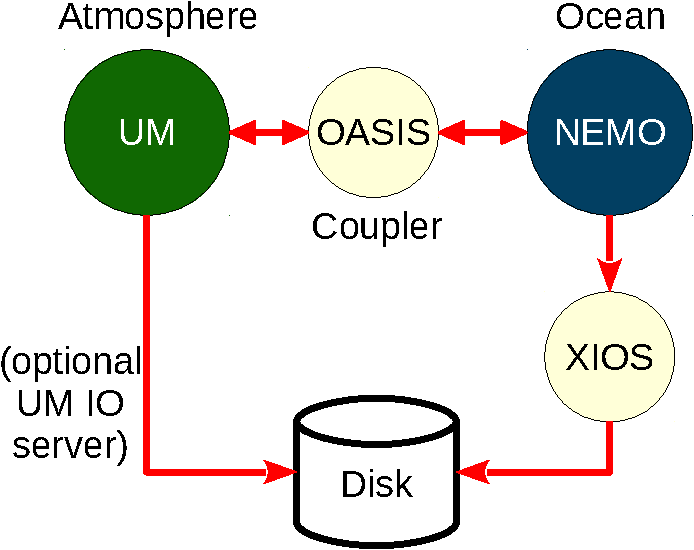
\includegraphics[scale=0.5]{figures/xios_figures_a.pdf}
	}
	\caption{Schematic of the existing UK climate mode.}
	\label{coupled}
\end{figure}

\subsection{The Unified Model}

Developed jointly by the Met Office, its partner organisations, and the academic climate and weather research community, the UM is the model chiefly used to run numerical simulations in the UK academic and research-centre environments. Much of this work is undertaken on ARCHER, accounting for ~2000 MAU annually. The model is run in a wide range of configurations varying from low-resolution, high-fidelity Earth System models (UKESM \cite{Ukesm}), to very high-resolution climate (PRIMAVERA), to ultra-high-resolution process studies (PARACON). The UM is an MPI-OMP code written in FORTRAN, with a small amount of C. The UM has very few software dependencies, principally the communications library (GCOM), which is simply a wrapper for MPL, and, depending on precisely how the model is configured, possible dependencies on NetCDF and HDF5. The UM is managed through a workflow system, which combines a model configuration system Rose \cite{Rose} and workflow scheduling engine Cylc \cite{Cylc}.

\subsubsection{Climate Configuration}
While the UM can be configured with time-varying sea-surface ancillary fields to mimic fully interactive atmosphere-ocean coupling, it is more commonly the case that a fully coupled configuration is employed. Figure \ref{coupled} outlines the components of the coupled model -- the UM (atmosphere) and NEMO (ocean) run asynchronously with a defined coupling frequency. Fields are exchanged between the two components using the OASIS coupler, which performs the required conservative regridding between UM (lat-long) and NEMO (tripolar) grids. The UM currently manages its output through its proprietary IO server scheme, and NEMO uses XIOS to output diagnostics (prognostics are handled differently.)

\begin{figure}
        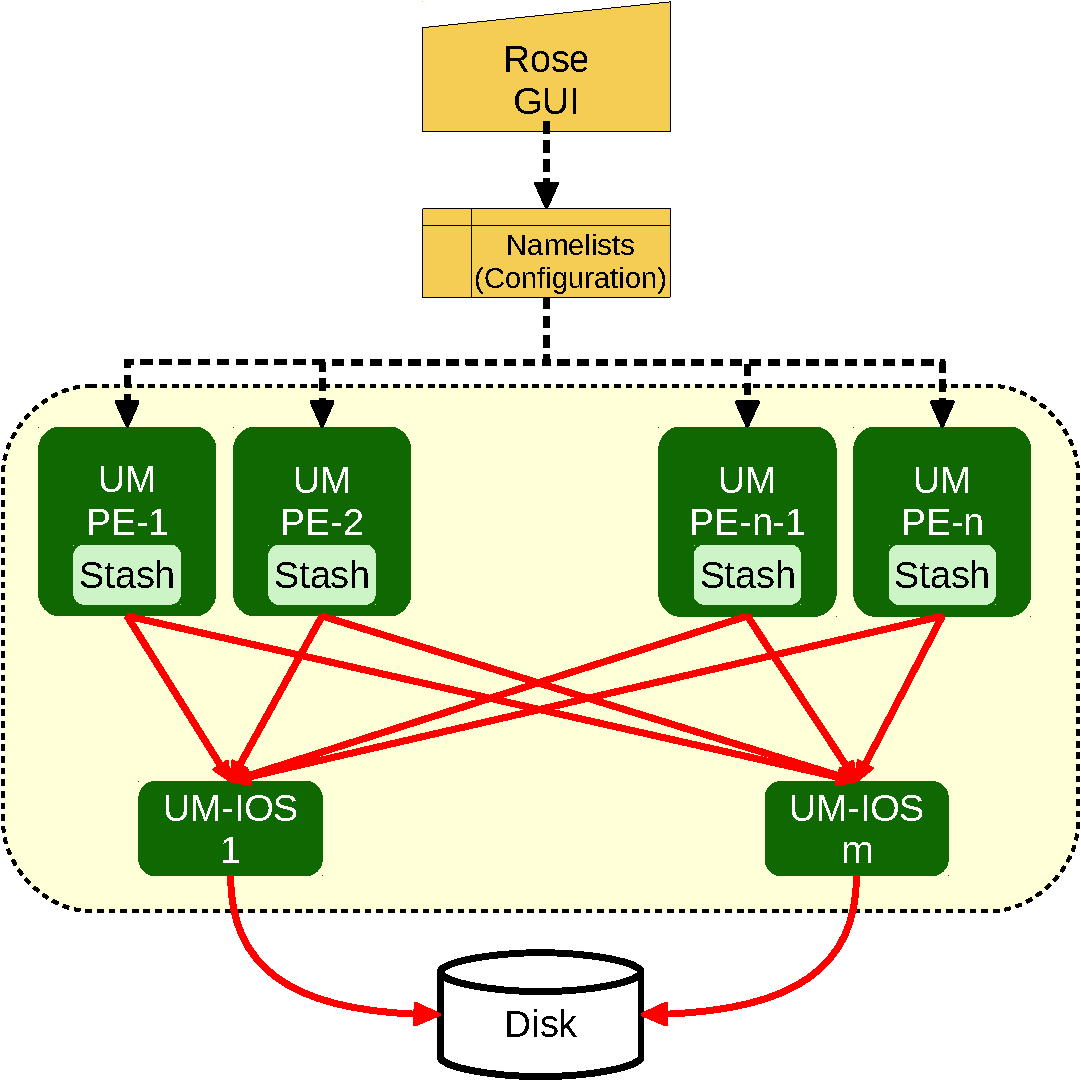
\includegraphics[width=\columnwidth]{figures/xios_figures_c.pdf}
        \caption{The Unified Model Configuration and output data flow (for an atmosphere only instance): configuration files define the domain decomposition (the number of processing elements, PEs) and the outputs required. Output is written to ``STASH'' and then, in the IO server configuration, written to multiple IO server instances, which each writes to disk. One MPI context (shown in yellow) covers the entire activity.
                Control flow is shown in black, data flow in red.
}
\label{uma-fig}
\end{figure}

\subsubsection{Current UM IO scheme}
The UM diagnostics system, commonly referred to as STASH, has been developed over 25 years into a highly configurable and versatile scheme for extracting and filtering UM fields. Recent advances have seen the successful development of CF-NetCDF capability circumventing the writing data in UM format. Diagnostics are made available for selection through the Rose GUI, where in addition, they can be configured for temporal and spatial processing. Rose generates FORTRAN namelists from user choices -- the workflow is sketched in Figure \ref{uma-fig} -- which are read at runtime to control model execution.
The UM IO scheme is a client-server model: diagnostics are processed and buffered on the compute PEs and then moved to the servers (UM-IOS in Figure \ref{uma-fig}) to be written to the disc. The number and placement of server processes are configurable.

\subsubsection{Resolution and Performance}
Climate models typically run at low or high resolution. Low resolution is designated as N96 with 96x2 zonal grid points for resolution of 135km at the equator; the high resolution is designated N512, which translates to 25km on the equator. We are currently running N1280 (5km) and developing N2560 (2.5km).

Figure \ref{scaling-um-fig} shows the results of some scaling runs for a high-resolution (N512) atmosphere-only climate model, which is essentially the model used throughout this work, on ARCHER and NEXCS (part of the MO Cray XC40), with and without IO. IO was managed through the UM IO servers (see Figure \ref{uma-fig}), which implement asynchronous IO to write data in the proprietary UM data format. The figure also shows scaling behaviour for a low-resolution model, which includes an expensive atmospheric chemistry scheme. All runs were performed with two OMP threads (required for the UM IO server). The N512 model scales reasonably well out to 15000 cores both and without IO -- changes to the IO profile can have a significant impact on performance through increased stalling resulting from inappropriate buffering or simply overmatching the machine IO bandwidth (recall that ARCHER is a very heavily loaded machine).) 


\begin{figure}
        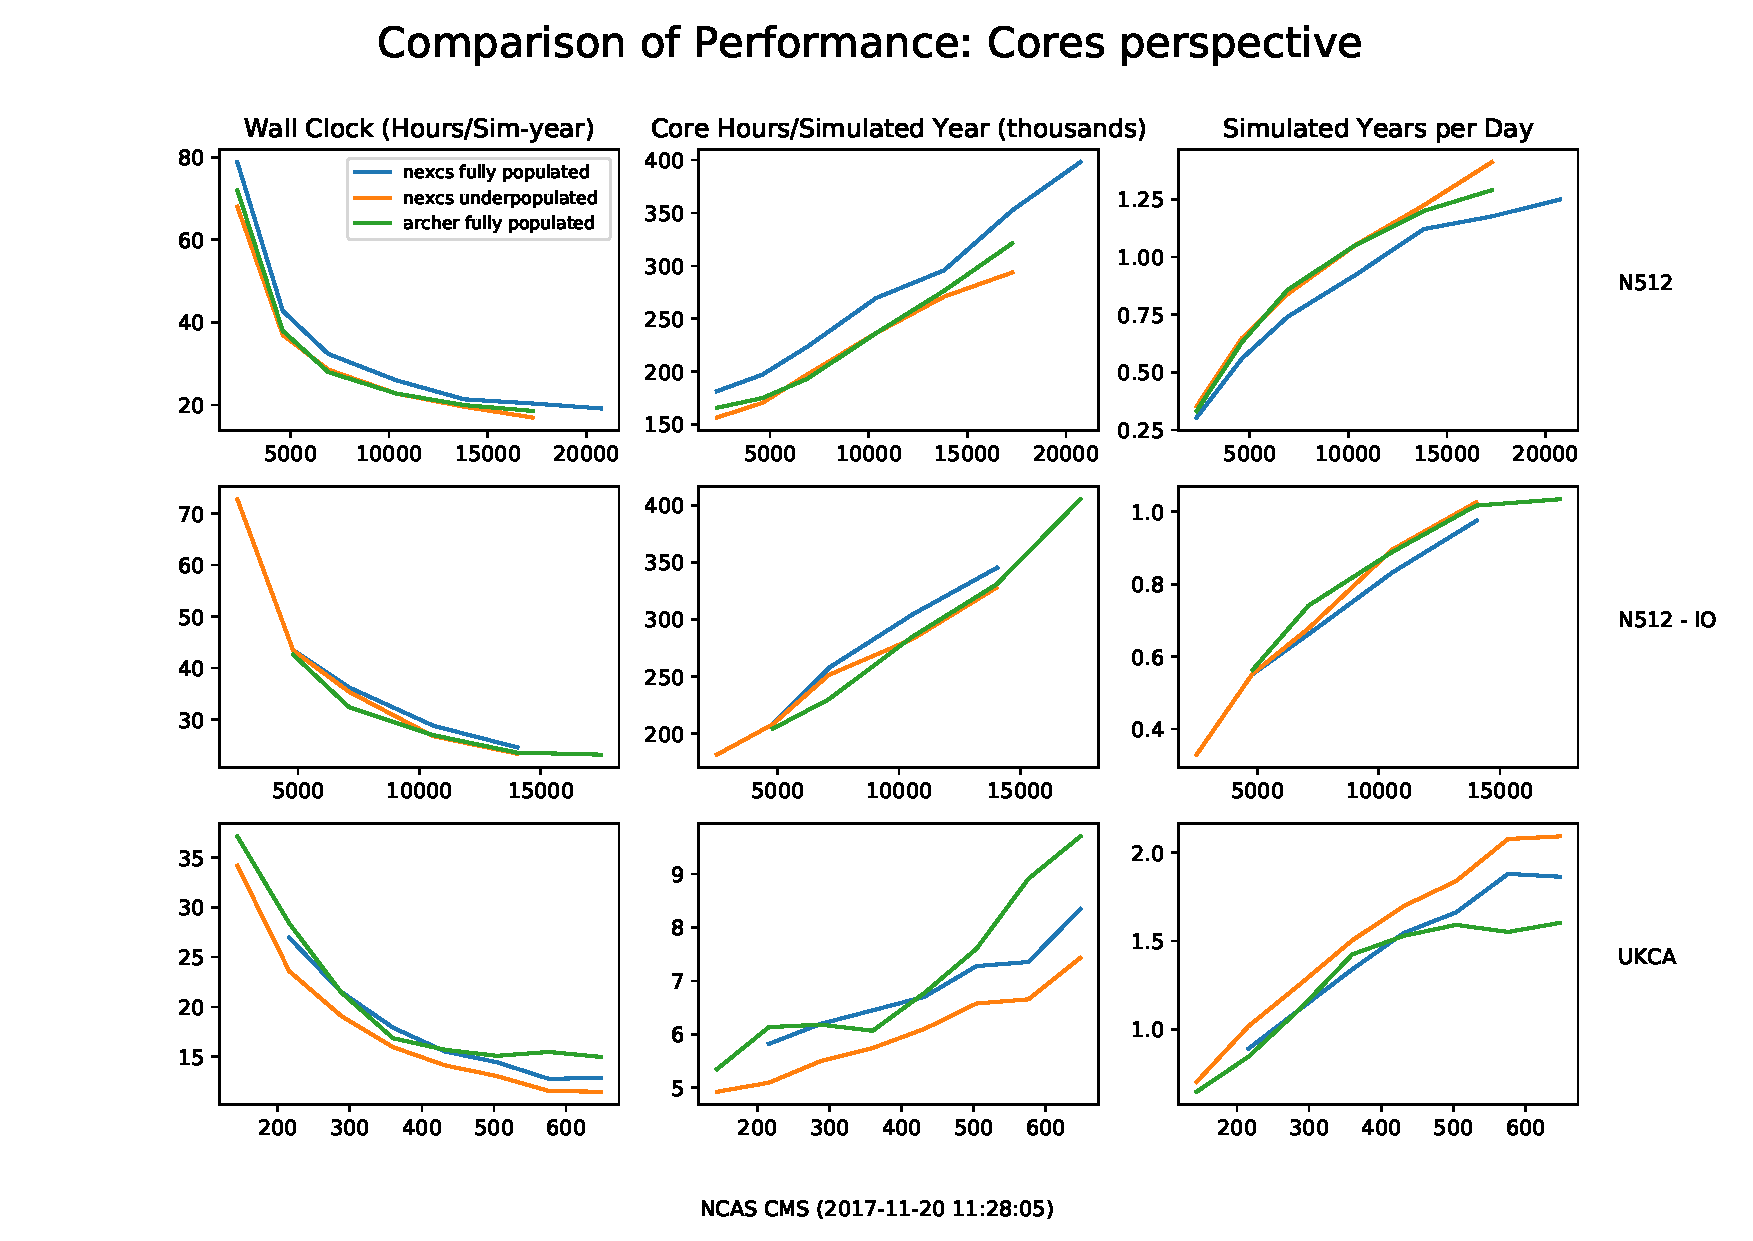
\includegraphics[width=\columnwidth]{figures/Cores.pdf}
        \caption{UM atmosphere strong scaling for a high resolution (N512) model with and without IO, and for a low resolution (N96) model with atmospheric chemistry included. All plots display wall clock time against number of cores.}
        \label{scaling-um-fig} 
\end{figure}



\subsection{XIOS}

XIOS (XML IO Server) is a software system developed at IPSL (Institute Pierre Simon Laplace) through IS-ENES (Infrastructure for the European Network of Earth System Modelling) \cite{Enes}, CONVERGENCE, ICOMEX, and ESiWACE \cite{Esiwace}. XIOS is organised around a hierarchical description of its data through an external XML file providing a simple interface for the user. XIOS offers dedicated servers for asynchronous output to overlap with computation, parallel IO for single file output and possible performance improvement and simplified downstream data workflow, in addition to multiple file (one per IO server) output. XIOS also offers the prospect of \textit{in situ} data analysis (our use of the phrase \textit{in flight} is based on this potential).  

XIOS is \~90,000 lines of C++; it is open-source software (under CeCiLL licence) and available at http://forge.ipsl.jussieu.fr/ioserver. The XIOS build system is based on FCM \cite{Fcm} with support for Intel and Cray compilers. We have built and run XIOS with Intel and Cray compilers. Our use of XIOS is based primarily on revision 1404.

XIOS is based on a client-server architecture, whereby each computer processor interacts with an XIOS client to expose agreed data fields through a minimalist interface. The set of fields to be exposed is defined by entries in the XML file. A simple FORTRAN call is all that the model needs to do to offload data to XIOS, thus:

\begin{verbatim}
call xios_send_field("field_id", field)
\end{verbatim}
where \texttt{"field\_id"} is a reference to the XML description of the field, which includes grid and domain information, and \texttt{field} is the address of the field data.

XIOS supports multiple data filters and transformations, including, importantly for this work, reductions over an axis.  


\subsubsection{XML}
The contents of the XML file are distinguished by \texttt{context}, which may represent a model or a component of a model. In the following XML snippet, we have defined the \texttt{atmosphere} context with associated XML elements referencing axis (typically the vertical or pressure axis in a climate model), domain (the horizontal structure), grid (combinations of domains and axes), field (specifying a set of \texttt{field\_id}s and their associated grids (a given \texttt{field\_id} can be output on multiple grids)), and file (specifying  output frequency, filename, other purely file-related criteria.) The XML file will typically comprise several contexts, each associated with a logically appropriate model or component.  

\begin{verbatim}
<simulation>
  <context id="atmospere" >
    <axis_definition   src="./axis_def.xml"  />
    <domain_definition src="./domain_def.xml"/>
    <grid_definition   src="./grid_def.xml"  />
    <field_definition  src="./field_def.xml" />
    <file_definition   src="./file_def.xml"  />
  </context>
  <context id="other" >
  ....
  </context>
</simulation>
\end{verbatim}

Judging from our experience with NEMO, the XML file is a very slowly changing object, i.e. model output is defined once and hardly changes over time. The use of XIOS in the UM research environment will require a much more quickly evolving XML configuration and the ability to easily modify it through methods incorporated into the well established UM model configuration infrastructure -- this is a must to ensure its acceptance by the UM community. 


\section{Software Structure}
\label{software}

There were four distinct software activities required to develop our ensemble system based on XIOS:
\begin{enumerate}
\item The XIOS system had to be inserted alongside the existing diagnostic system (we did not in these experiments completely replace the existing diagnostic system) 
\item We had to work out how to get XIOS to deliver ensemble statistics,
\item We had to work out how to get XIOS to control the ensemble,
\item We had to develop methods for configuring the model ensemble system to request the required diagnostics.
\end{enumerate}


\begin{figure}
	\centerline{
		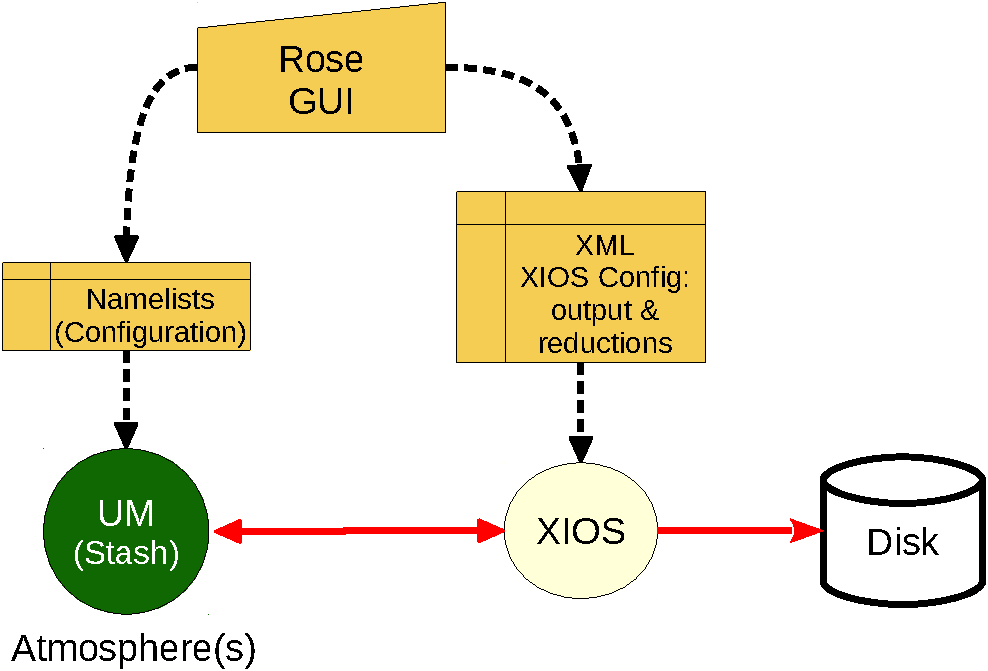
\includegraphics[scale=0.5]{figures/xios_config.pdf}
	}
	\caption{Maintaining the look and feel of UM diagnostics: the Rose GUI is used to configure both the UM atmosphere via namelists and the XIOS output. The UM reads the XML files and integrates them with the STASH system, and sends the fields to the XIOS server.} \label{fig-xconfig}
\end{figure}





\subsection{XIOS in the UM}

Given the maturity of the Rose system and its familiarity in the UM user community, it was essential that we did not develop a new diagnostic interface. Instead, our goal was to maintain the look and feel of the current system to enable easy user uptake of the new XIOS functionality. Figure \ref{fig-xconfig} shows the steps to achieve our objective. First, the diagnostic choices must be translated into an XML format to be read by XIOS, and the UM must be modified to hand off data to XIOS. 
\subsubsection{STASH to XML utility}
\label{stash2xml}
\begin{figure}
	\centerline{
	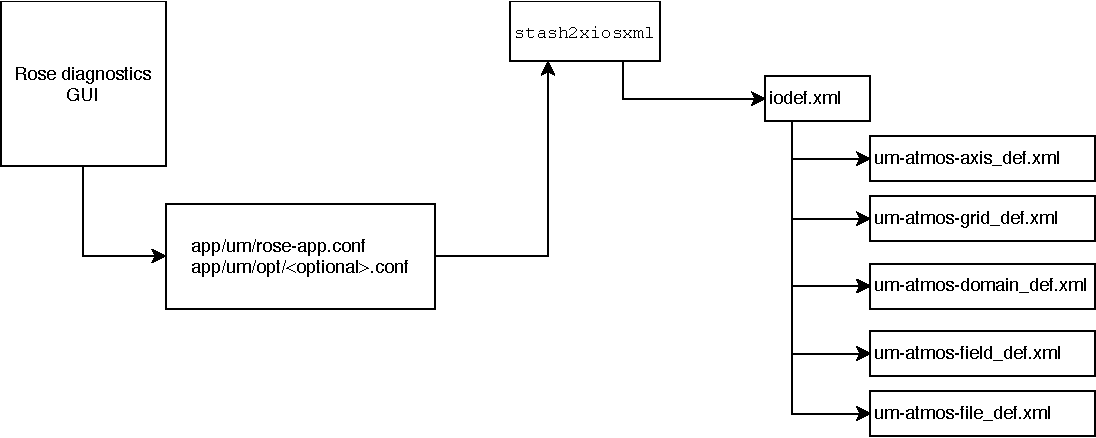
\includegraphics[scale=0.5]{figures/stash2xiosxml.pdf}}
	\caption {
                Workflow for creating XML files from STASH requests. The familiar Rose GUI isolates the user from details about XIOS XML. \texttt{stash2xiosxml} reads configuration files generated by Rose to create an XML description of the diagnostic output.
		}\label{stash2xiosxml}
\end{figure}
UM diagnostics are selected and configured through a Rose interface. The user selects a diagnostic and associates it with three ``profiles'': time, domain, and usage. The time and domain profiles represent specifications for temporal and spatial processing for the selected diagnostic (time meaning or accumulation, spatial meaning, or subspacing, for example); the usage profile, which, in combination with an output stream, determines the file structure for the diagnostic. We wished to maintain the routine diagnostics interface with XIOS; this was achieved by adding XIOS output streams to complement regular UM output streams and developing a utility to identify diagnostics destined for XIOS and translate their traditional STASH description into XML. 

We have developed \texttt{stash2xiosxml} to make the translation. 
\texttt{stash2xiosxml} is a Python utility that loads Rose suite configuration files into a hierarchical data structure, extracts and collates information relevant for XIOS diagnostics, cross-references with data held in the STASHMaster file to retrieve grid information, and writes the XML. Figure \ref{stash2xiosxml} is a schematic of the steps involved in XML creation; Rose creates possibly many configuration files which are inputs to \texttt{stash2xiosxml}; the XIOS standard XML file iodef.xml is output along with its subcomponents. 

Of the 4017 possible diagnostics available to a standard atmosphere UM model, we can handle the 3672, which are available on the main model time step. Diagnostics available on other time steps (the radiation time step, for example, which is typically a large multiple of the model time step) need special handling and are not covered in this work.


\subsubsection{New code in the UM} 
\label{new-code}
Files added to the UM named with the prefix \texttt{um\_xios} represent new code. The additional files are located in \texttt{/um/src/control/xios} and comprise approximately 3000 lines of code. Figure \ref{um-xios-code} indicates where the new code impacts the UM. Most work is done in the model initialisation stages, with only minimal changes required to intercept and redirect diagnostics to XIOS. The global communicator is split by a native XIOS call in \texttt{um\_xios\_init\_mpi} which returns the communicator for use by the model. The additional XIOS functionality is entirely independent of all other UM IO. Checkpoint files, logging files, and any diagnostics selected not to use XIOS are handled through traditional UM means.

\begin{figure}
	\centerline{
	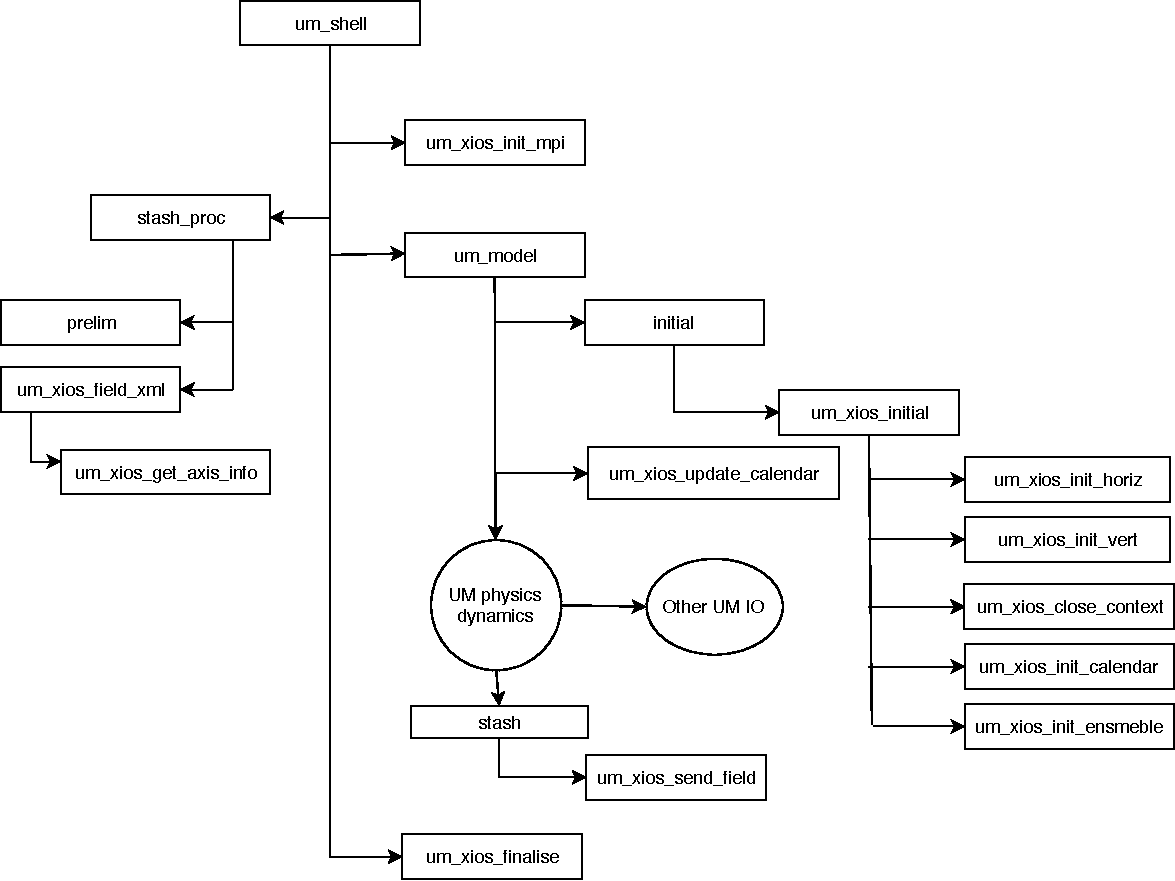
\includegraphics[scale=0.5]{figures/UM-XIOS-code.pdf}}
	\caption {
                Areas in the UM where the use of XIOS impacts the code. Diagnostics are intercepted in the routine stash. All other UM IO (logging, checkpointing, and diagnostics not directed to XIOS) is handled traditionally.
		}\label{um-xios-code}
\end{figure}


\subsubsection{Build system and job submission} 
Minor changes were made to the Rose GUI and the UM build configuration files to accommodate the use of the XIOS library. 
Minor changes were made to the Rose GUI and the scripts which generate the job submission file to enable the launch of the UM and XIOS in MPMD mode. 


\section{XIOS UM ensemble}
\label{um-ensemble}


In order to take full advantage of the existing XIOS reduction capabilities, we introduced the idea of the \textit{ensemble axis}. This novelty simply attaches an extra dimension to the data generated by the ensemble to indicate to which ensemble member a particular field belongs. This addition greatly simplifies \texttt{context} management in XIOS, since now the entire ensemble is associated with a single \texttt{context} -- XIOS simply sees an (n+1)-dimensional data set for the ensemble, where for a single model, it saw an n-dimensional data set. Applying reductions over the ensemble axis provides the mechanism for generating ensemble statistics.

Figure \ref{fig-xios-layout} describes the key features of our XIOS UM ensemble configuration. From the XIOS viewpoint, the UM ensemble is simply a model -- XIOS clients reside on each PE and send fields to XIOS servers. An individual ensemble member runs in its familiar environment -- exactly as before.

Several XML files are augmented for the ensemble case; the additional ensemble axis feeds through to ensemble XML grid, and file definitions. An ensemble grid would appear thus:

\begin{verbatim}
<grid_definition>
  <grid id="um-atmos_grid">
    <domain domain_ref="um-atmos_domain" />
    <axis axis_ref="um-atmos_vertical" />
    <axis axis_ref="ensemble" />
  </grid>
</grid_definition>
\end{verbatim}
Attaching this grid to a field will result in its output of data for all ensemble members.

\subsection{UM code for an ensemble}

For the ensemble case, the model communicator provided by \texttt{um\_xios\_init\_mpi} (see section \ref{new-code}) is split again for each ensemble member. Individual ensemble member models run on their own model communicators, and as previously for the single model case, non-XIOS IO (read and write input, logging files, checkpoints...) are handled in their own separate ensemble-member spaces. 

Other than additions to \texttt{whatroutine} to ensure that each member executable runs in a specific directory (a requirement imposed by the Rose infrastructure) and minor additions to accommodate setting up the ensemble axis, the code described in Figure \ref{um-xios-code} suffices for the ensemble case.

\begin{figure}
	\centerline{
	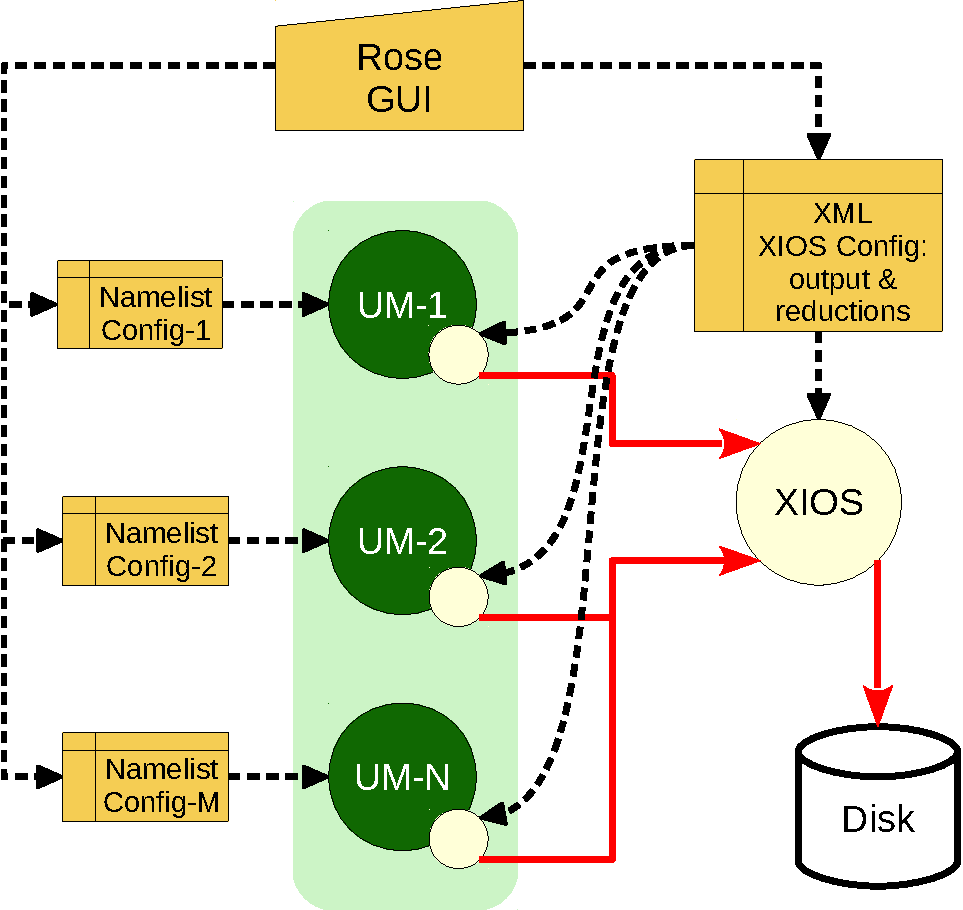
\includegraphics[scale=0.5]{figures/xios_figures_b.pdf}}
	\caption {
		Key control and data flow concepts for XIOS control of a UM ensemble. The XIOS controls
		the output of each UM instance by exploiting
		XIOS clients within each process of each UM instance. Output from the clients goes through
		XIOS server instances to disk. 
		}\label{fig-xios-layout}/
\end{figure}

\subsection{Rose ensemble configuration}

As set up through Rose, a UM simulation is defined as a collection of configuration files (in INI format). On job submission, (i) Rose creates namelists from the configuration files; (ii) creates a workspace on the HPC; (iii) copies the namelists (and other data) into the workspace; (iv) sets up and submits a PBS script to run the parallel job. We have developed a Rose ensemble member setup task to perform items (i)-(iii), which, in conjunction with the use of Rose optional override configuration files to specify parameters for each ensemble member, create the appropriate environment for each member to run in on the HPC. An override file typically contains one line to set an initial condition or a parameter value. 

A separate task to run the ensemble then creates the appropriate MPMD aprun command for submitting multiple UM instances and XIOS.


\subsection{Configuring ensemble output}

XIOS currently supports max, min, and mean reductions. Our interest is primarily in the ensemble mean. It is a general feature of XIOS that data transformations are performed based on the target grid for the output field. In the example in section \ref{um-ensemble}, the target grid spanned all ensemble members; a reduction over the ensemble axis is achieved by appropriately defining the grid on which to output the field. In the following, the ensemble-reduction grid \texttt{um-atmos\_grid-reduce} includes instruction to reduce over the ensemble axis with operation \texttt{average}.

\begin{verbatim}
 <grid id="um-atmos_grid-reduce">
    <domain domain_ref="um-atmos_domain" />
    <axis axis_ref="um-atmos_vertical" />
    <scalar id="3d-ensmean">
      <reduce_axis operation="average" />
    </scalar>
  </grid>
\end{verbatim}
Our Python utility \texttt{stash2xiosxml} (section \ref{stash2xml}) includes support for creating XML for ensemble reductions.


\section{Results}
\label{results}

Our underlying UM configuration is GA7.0 UM 11.4 AMIP \cite{Modelconfig} which we run at both low resolution (N96) and high resolution (N512) in conjunction with XIOS at revision 1740. The model was configured to run for 46 model hours, with data output two-hourly. In addition, we selected diagnostics from several UM physics and dynamics sections, output as instantaneous fields for a total of 40 fields (28 fully 3d, two 2d, ten on a reduced set of pressure levels), with the aim to mimic typical near-future climate integration data volumes, though clearly not representative of the potentially bursty profile of climate output. 

\subsection{Single UM}

An essential requirement for an IO (or more appropriately, a diagnostics) server is that it is capable of managing its activity (data processing and writing to disc) asynchronously and without stalling or throttling the main computation (keeping 50,000 processors idle while data is written to disc is an expensive prospect). Our main single UM test focused on confirming that XIOS can handle large amounts of data without impacting model computation times. Our high-resolution configuration creates 165GB of data/model day, which translates to 59TB/model year, which exceeds our current N512 production output rate by a factor of 30. XIOS provides many opportunities for performance optimisations that we have not explored. Nevertheless, the results in Table \ref{table3} with 30 XIOS servers in multiple-file mode indicate that XIOS is effectively hiding IO from the computation. The 2\% XIOS overhead is an acceptable penalty for the rate of data production seen here. Single file output can incur a more significant IO overhead and requires more tuning for optimal performance, which is out of scope here, and perhaps of less interest in the longer term with the increased interest in data sharding and the ongoing developments in data analysis techniques. \cite{NEEDED}.

\begin{table}
	\begin{center}
	\begin{tabular}{|l|r|}
		\hline
		Resolution & \multicolumn{1}{c|}{PEs} \\
		\hline
		N96 & 504\\
		N512 &1920 \\
		\hline
	\end{tabular}
	\caption{Single model core counts}
        \label{table1}
	\end{center}
\end{table}
 

\subsection{UM ensembles}

We applied our developments to ensembles of N96 and N512 models. Results from our initial experiments are presented in Figures \ref{first-ensemble-runs-n96} and \ref{first-ensemble-runs-n512}. We have removed all one-time costs from the timings reported here, including times for initialisation and finalisation of the UM ensemble and XIOS. Data points in red represent the sum of times for each model time step measured by UM timers and include XIOS overheads. Data points in blue represent the average time per output time step (non-output time steps take the same time irrespective of ensemble size, as expected) and indicate the extra time XIOS needs to perform the ensemble averaging.

 This configuration is not how we anticipate production runs to work but serves as a robust test case.

\subsubsection{N96}

The multiple-file ensemble performance is encouraging with relatively flat performance over the range of ensemble sizes -- horizontal lines represent perfect performance. Although not reported here, the time for an output time step strongly depends on the number of IO servers used for the run; the 50-member ensemble with 6 IO servers runs with an average output time step time of ~17s. The run reported here used 20 IO servers. However, we shall not be concerned with the number of IO servers since they constitute a small component of the entire ensemble resource requirement. 



\subsubsection{N512}

Memory requirements on the XIOS clients limited the maximum size of the N512 ensemble. Given our choice of output fields, a maximum of 15 ensemble members enabled an acceptable turnaround on ARCHER. All our test cases ran with 30 IO servers. AS for the N96 case, it is clear that the overhead for generating ensemble averages increases linearly with ensemble size and constitutes a slight increase in the ensemble run time.



\begin{table}
	\begin{center}
	\begin{tabular}{|l|r|r|}
		\hline
		Resolution & \multicolumn{2}{c|}{Ensemble Size} \\
		 & 100 & 15 \\ \hline
		N96 & 50400 & \\
		N512 & & 28800 \\
		\hline
	\end{tabular}
	\caption{Maximum core counts for the largest ensembles}
        \label{table2}
	\end{center}
\end{table}

\begin{table}
	\begin{center}
	\begin{tabular}{|l|r|r|r|r}
		\hline
		 & no IO & XIOS & UM IO (single PE) \\
		\hline
		run time     & 1486 & 1520 & 2860\\
                IO overhead  &     & 34  & 1374\\
		\hline
	\end{tabular}
	\caption{Single model N512 IO performance. The integration ran for 46 model hours to create 330GB of diagnostic output (equivalent to 59TB/year.) The significant IO overhead (~92\%) for a synchronous write is reduced to ~2\% when XIOS is used. All times in seconds and model initialisation and finalisation time removed.  }
        \label{table3}
	\end{center}
\end{table}

\begin{figure}
	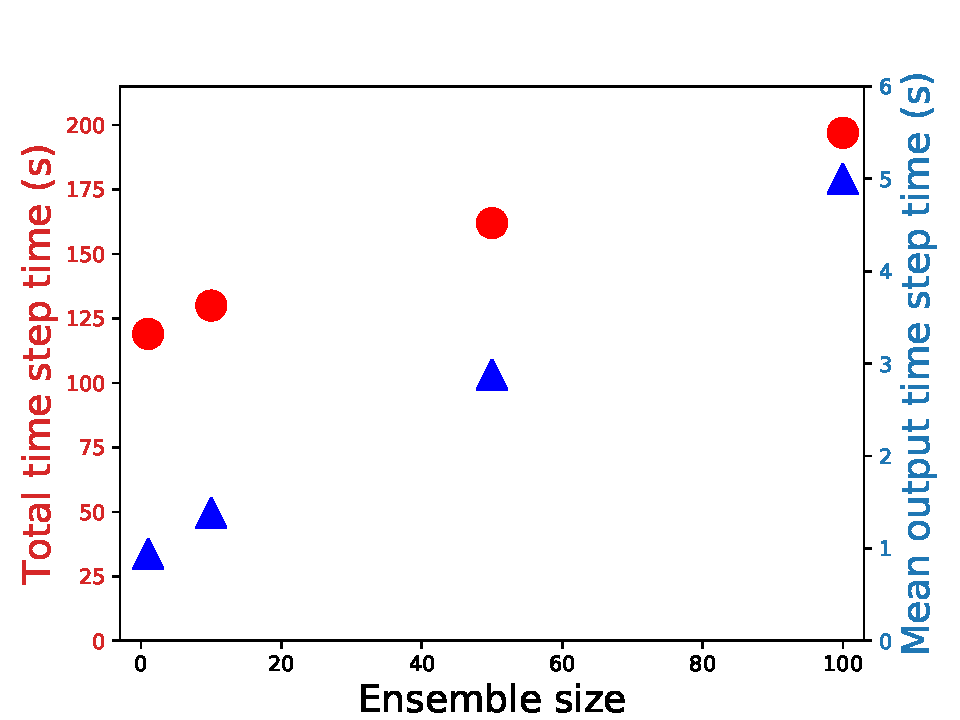
\includegraphics[width=\columnwidth]{figures/ens-n96.pdf}
	\caption{Scaling curves for ensemble writing using N96 ensembles for multiple file output. Each N96 ensemble member ran on 504 PEs. Red data points represent the sum of times per time step for the run; the model performs ensemble averaging and data output every 6th-time step. The blue data points represent the average time for the output time step, which exhibits a near-linear scaling with ensemble size.}
        \label{first-ensemble-runs-n96}
\end{figure}

\begin{figure}
	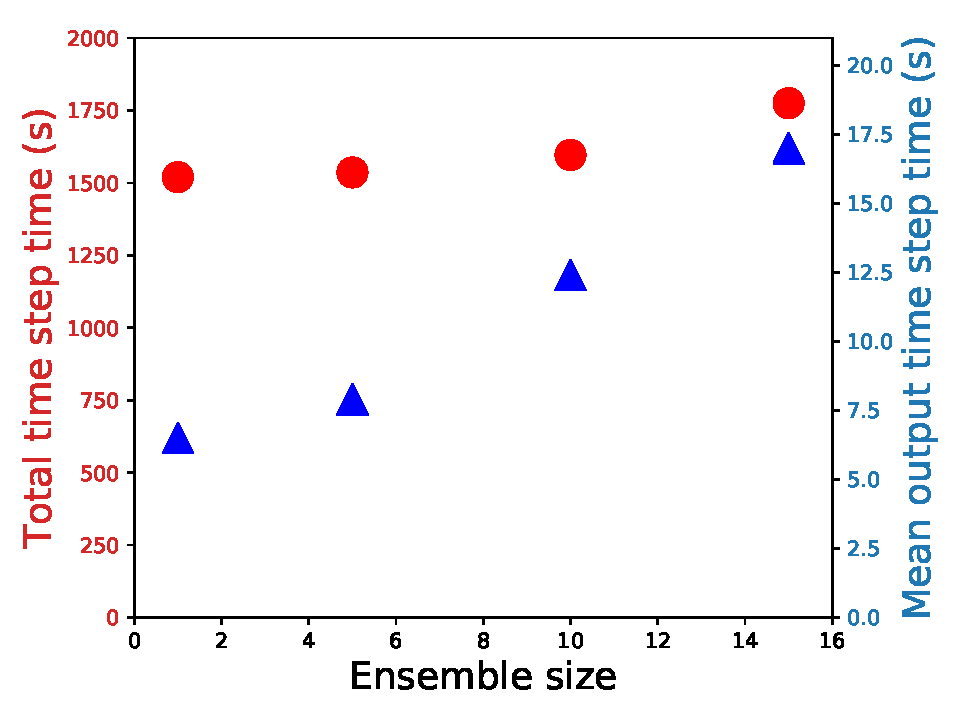
\includegraphics[width=\columnwidth]{figures/ens-n512.pdf}
	\caption{Scaling curves for ensemble writing using N512 multiple file output. Each N512 ensemble member ran on 1920 PEs. Red data points represent the sum of times per time step for the run; the model performs ensemble averaging and data output every 12th-time step.The blue data points represent the average time for the output time step, which exhibits a near-linear scaling with ensemble size.}
        \label{first-ensemble-runs-n512}
\end{figure}



\section{Summary and Further Work}
\label{summary}

We have achieved three specific ambitions: (1) We have adapted a current Met Office Unified Model branch to replace much of the diagnostic system with the XIOS.
(2) We have exploited a single executable MPI environment to run multiple UM instances with output sent to XIOS, and (3) We have demonstrated that simple ensemble statistics can be calculated in-flight, including both summary statistics of individual ensemble members and cross-member statistics such as means and extremes.

In our current setup, failure of a single ensemble member will crash the entire ensemble; we have inherited UM checkpointing, of course, so restarting the ensemble is possible, but ideally, we should be able to manage such a failure more gracefully. For example, we can imagine a scenario whereby we would trap ensemble member errors and subsequently send \textit{missing data} or otherwise signal the failure to XIOS; a modified XIOS would handle the situation in a manner to be determined. 

There is scope to improve the range of ensemble processing capability within XIOS significantly and indeed in the entire ensemble management activity.

We note that the Met Office have expressed an interest in assisting us in putting our UM branch into a UM release in light of our successes and view of their anticipated use of XIOS in LFric \cite{Lfric}.





\clearpage

\section*{Acknowledgements}

This work uses the ARCHER UK National Supercomputing Service (\url{http://www.archer2.ac.uk}). This work is funded under the embedded CSE programme of the ARCHER UK National Supercomputing Service (\url{https://www.archer2.ac.uk/ecse}). 
We thank Yann Meurdesoif for assisting us with all aspects of XIOS.


We also acknowledge support from NCAS.

\section*{References}

\bibliography{ensembles18}
\bibliographystyle{elsarticle-num}



\end{document}
